% !TEX program = pdflatex
%%%%%%%%%%%%%%%%%%%%%%%%%%%%%%%%%%%%%%%%%
% Structured General Purpose Assignment
% LaTeX Template
%
% This template has been downloaded from:
% http://www.latextemplates.com
%
% Original author:
% Ted Pavlic (http://www.tedpavlic.com)
%
% Note:
% The \lipsum[#] commands throughout this template generate dummy text
% to fill the template out. These commands should all be removed when
% writing assignment content.
%
%%%%%%%%%%%%%%%%%%%%%%%%%%%%%%%%%%%%%%%%%

%----------------------------------------------------------------------------------------
%	PACKAGES AND OTHER DOCUMENT CONFIGURATIONS
%----------------------------------------------------------------------------------------

\documentclass{article}

\usepackage{fancyhdr} % Required for custom headers
\usepackage{lastpage} % Required to determine the last page for the footer
\usepackage{extramarks} % Required for headers and footers
\usepackage{graphicx} % Required to insert images
\usepackage{subcaption}
\usepackage{lipsum} % Used for inserting dummy 'Lorem ipsum' text into the template

\usepackage[utf8]{inputenc}
\usepackage[ngerman,english]{babel}
\usepackage[T1]{fontenc}
\usepackage{breakurl}
\usepackage[hyphens]{url}
\usepackage{color}
\usepackage{float}
\usepackage[hidelinks]{hyperref}
\usepackage{tabularx}
\usepackage{enumitem}
\usepackage{color, colortbl}
\usepackage[super]{nth}
\usepackage{wrapfig}
\usepackage{amsmath}
\usepackage{amssymb}
\usepackage{booktabs}

\usepackage[
	backend=biber,
	style=numeric-comp,
	natbib=true,
	url=false,
	doi=false,
	eprint=false,
	sorting=none,
	isbn=false]
	{biblatex}

\bibliography{references}

\addto\captionsenglish{%
  \renewcommand{\contentsname}%
    {Table of Contents}%
}

% Margins
\topmargin=-0.45in
\evensidemargin=0in
\oddsidemargin=0in
\textwidth=6.5in
\textheight=9.0in
\headsep=0.25in

\linespread{1.1} % Line spacing
% Set up the header and footer
\pagestyle{fancy}
\lhead{} % Top left header
\chead{} % Top center header
\rhead{\firstxmark} % Top right header
\lfoot{\lastxmark} % Bottom left footer
\cfoot{} % Bottom center footer
\rfoot{Page\ \thepage\ of~\pageref{LastPage}} % Bottom right footer
\renewcommand\headrulewidth{0.4pt} % Size of the header rule
\renewcommand\footrulewidth{0.4pt} % Size of the footer rule

\setlength\parindent{0pt} % Removes all indentation from paragraphs

\begin{document}
\setcounter{tocdepth}{2} % No subsubsections


%----------------------------------------------------------------------------------------
% TITLE PAGE
%----------------------------------------------------------------------------------------
\pagenumbering{gobble}
% \maketitle
\begin{titlepage}
  \centering
\includegraphics[width=5cm]{figures/tumlogo}

  \vspace{2.5cm}
  \Huge{Network Security} \\
  \vspace{0.1in}\huge{Summary}\\

  \Large
  \vspace{1.5cm}
  \begin{tabularx}{9cm}{r l}
    Author: & Thomas Pettinger\\
  \end{tabularx}

  \vfill
  \textbf{2017--03--02} \\
  \vspace{0.3in}\normalsize{Network Security}\\
  \vspace{0.03in}\normalsize{\textsc{Technische Universität München}}\\
  \vspace{1cm}

\end{titlepage}
%----------------------------------------------------------------------------------------


\newpage
\thispagestyle{empty}
\tableofcontents

\newpage
\pagenumbering{arabic}

%!TEX root = ../report.tex

\section{Introduction}

\subsection{Attacks and Attack Detection}
Attacks can have different impacts on the target.
Disruptive attacks try to fully deny the service (DoS) of the victim whereas degrading ones only occupy parts of the resources.
A DoS attack can also executed distributed, a so called DDoS.
Attackers might also try to gain confidential data or control the target system.
Port scans can be used to gain information about the network topology, operating systems and applications or application versions.\\

To be able to tell if a system is under attack, different measures can be taken at different points in the system.\\
Host intrusion detection systems (HIDS) are located on the host system.
This enables easy detection using information available on the potential victim system but it has to be present on every system (expensive deployment) and the attack actually reaches the victim and is not detected in advance.
Network intrusion detection systems (NIDS) lay on the network layer which enables the detection of attacks before they reach the host.\\
One of the detection methods available is knowledge-based detection.
Known signatures of attacks are compared to the actual traffic and if the patterns match an alarm is raised.
This only detects known attacks though.
To improve this shortcoming, anomaly detection in traffic, protocol or applciaiton behavior can be used.
Anomalies can be detected with different metrics in mind.
A very simple one might be the number of request, but this does not take legitimate change in traffic into account.
A better approach is using cumulative sums which are low if the average is small or whenever only small amounts of values are large but grows if the amount of large values grows in a certain point in time.
The disadvantage of anomaly detection though is that oftentimes the rate of false-positives is high.\\
Detecting attacks is not easy and network monitory often comes at a cost.
It is important though especially in large systems when the attack surface grows.
The challenge is to find a good compromise between security and performance.

\subsection{Attacker Model and Locations}
We generally assume the attacker to be (in) the network.
They can perform any active or passive attack but cannot break cryptographic primitives.
Active attacks are attacks where some influence is measurable e.g.\ a delay, modifications or replays whereas a passive attack simply stands for eavesdropping messages.
This model is called the Dolev-Yao attacker model.\\

Attackers can be located on different parts of the network and depending on this location different attacks are possible.
If the attacker is close to you they are able to perform active attacks like message modifications on you.
This can be circumvented by communicating over a secure tunnel though.
If the attacker is close to your servers, timing attacks are possible where attackers can measure how long certain operations take to break into the system.
The last possibility is that the attacker is somewhere in the Internet.
Since the end user has no control over how packets are routed, attackers can modify the path they take for example.

\subsection{Security Goals}
\begin{description}
  \item[Data Integrity] No improper or unauthorized change of data
  \item[Confidentiality] Concealment of information
  \item[Availability] Services should be available and function correctly
  \item[Authenticity] Entity is who she claims to be
  \item[Accountability] Identify the entity responsible for any communication event
  \item[Controlled Access] Only authorized entities can access certain services or information
\end{description}

\subsection{Threads}
We define a thread in a communication as any possible event or sequence of actions that might lead to a violation of one or more security goals.
The actual realization of a thread is then called attack.\\

Different threads are possible:
\begin{itemize}[noitemsep, topsep=0pt]
  \item \textbf{Masquerade}: An entity claims to be another entity (also called ``impersonation'')
  \item \textbf{Eavesdropping}: An entity reads information it is not intended to read
  \item \textbf{Loss or Modification of (transmitted) Information}: Data is being altered or destroyed
  \item \textbf{Denial of Communication Acts (Repudiation)}: An entity falsely denies its participation in a communication act
  \item \textbf{Forgery of Information}: An entity creates new information in the name of another entity
  \item \textbf{Sabotage/Denial of Service}: Any action that aims to reduce the availability and / or correct functioning of services or systems
  \item \textbf{Authorization Violation:}: An entity uses a service or resources it is not intended to use
\end{itemize}

\newpage

%!TEX root = ../report.tex

\section{Language-theoretic Security}
Communication protocols define the procedure and the format of exchanged messages.
If two communication partners speak the same protocol it is not necessarily given that they have the same understanding though.
Different problems may arise which result in some guidelines to avoid them:

\begin{description}
  \item[Full input recognition] Programmers usually assume well formed input where in reality the input is controlled by the attacker.
    For this reason every input should be checked if it fulfills the expectations of valid inputs.
  \item[Only Type 2 or 3 of Chomsky Hierarchy grammars for inputs]
    Do not define turing-complete protocols because recognition of the input and testing the equivalence of implementations is undecidable.
    \begin{figure}[h]
      \centering
      \begin{tabular}{l l l}
        Grammar & Language & Recognized by\\
        \midrule
        Type 3 & Regular & Finite state automaton\\
        Type 2 & Context-free & Pushdown automaton\\
        Type 1 & Context-sensitive & Some weird stuff\\
        Type 0 & recursively enumerable & Turing machine\\
      \end{tabular}
      \caption{Chomsky Hierarchy of Languages}
    \end{figure}
  \item[Reduce computing power] Reduce the computing power exposed to the outside.
    Computing power that is not there can not be exploited.
    This also includes defining protocols only in type 2 or 3 languages since parsing types 0 and 1 requires large or potentially unlimited amounts of computing.
  \item[Same interpretation of messages] All participants of a communication should interpret messages the same way.
    For this parsers have to be equivalent which is only decidable for type 2 and 3.
\end{description}


\newpage

%!TEX root = ../report.tex

\section{Firewalls and Security Policies}
We define a system as secure if, started in an allowed state, always stays in states that are allowed.

\subsection{The three Security Components}
\begin{itemize}
  \item \textbf{Requirements} define security goals
  \item \textbf{Policy} are rules to implement the requirements
  \item \textbf{Mechanisms} enforce the policy
\end{itemize}

\subsection{Network Firewalls}
Firewalls provide \textbf{controlled access} at the network level to resources.
They are usually deployed where a protected subnet is connected to a less trusted network like the internet (c.f.\ Figure~\ref{fig:firewall_placement}).
From the firewall's point of view, there are incoming and outgoing packages on all interfaces.
These can be filtered using two different strategies.\\
\textbf{Whitelisting}, which is considered as the best practice, has the default behavior of denying all packets and allowing only explicitly permitted ones whereas \textbf{blacklisting} allows everything except blocked packets.


\begin{figure}[h]
  \centering
  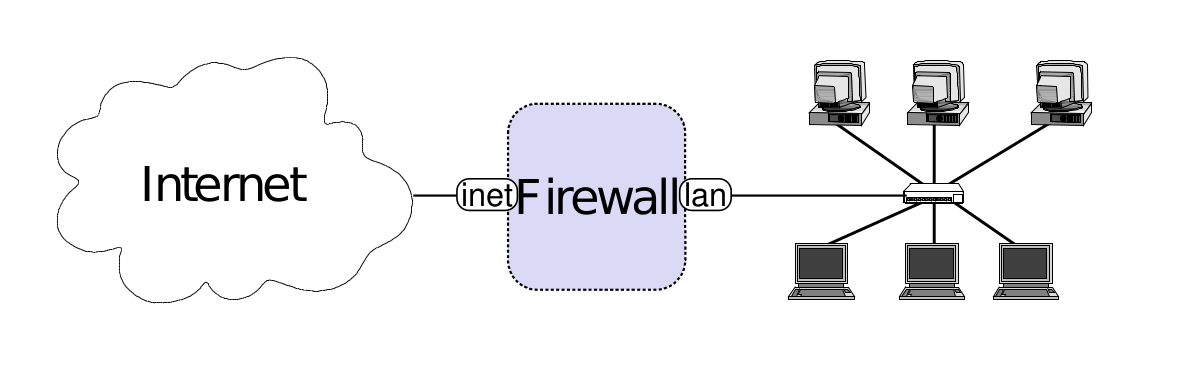
\includegraphics[width=.8\textwidth]{figures/firewall_placement.png}
  \caption{Firewall Placement}\label{fig:firewall_placement}
\end{figure}

\subsubsection*{Configuring Firewalls}
Firewalls are configured with rulesets which are traversed sequentially until a matching one is found.
Those rules are composed of a matching condition and an action.
Possible actions are for example accept, drop, reject or log.
The matching conditions are a bit more complex.
They include the incoming interface, several layer 2 to 4 packet fields (srcMAC, dstMAC, srcIP, dstIP, prot, srcPort, dstPort, flags,\dots), states (in case of stateful matching) and other relevant conditions.

\subsubsection*{Stateful Firewalls}
Stateful Firewalls keep states of connections with the help of IP-5-Tuples (srcIP, dstIP, protocol, srcPort, dstPort).
A new state is generated when a packet with a new tuple arrives which transitions from NEW to ESTABLISHED state.
It is usually advisable to put more frequently used rules to the top of the firewall, i.e.\ matching established connections (new connections are rarer) and to check that ports are above the well defined port range ($\geq 1024$).
Figure~\ref{fig:stateful_firewall} shows an example of a stateful firewall configuration.
\begin{figure}[h]
  \centering
  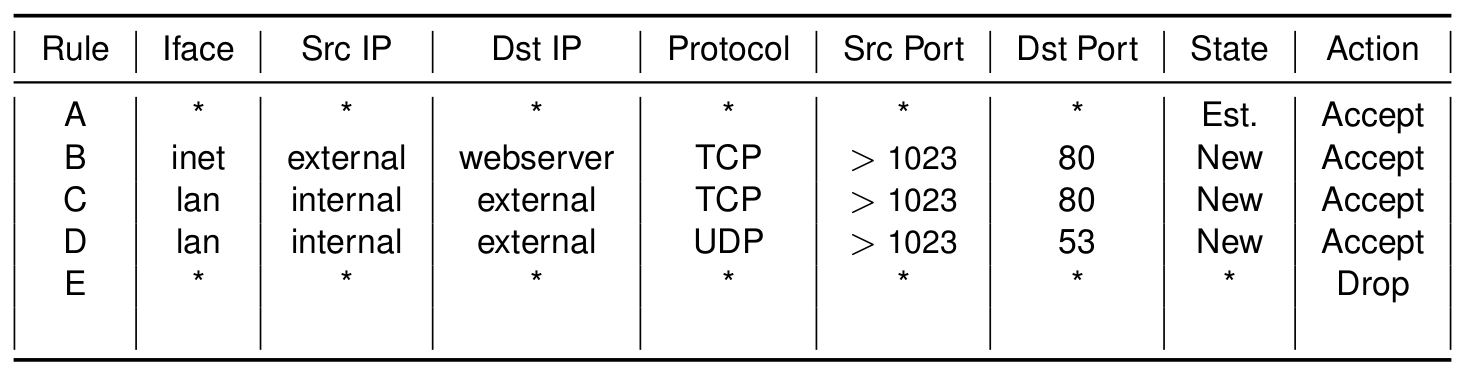
\includegraphics[width=.8\textwidth]{figures/stateful_firewall.png}
  \caption{Stateful Firewall Configuration}\label{fig:stateful_firewall}
\end{figure}

\subsubsection*{Stateless Firewalls}
Stateless firewalls do not generate states for incoming connections but only operate on single packets since keeping states is expensive and needs fast memory.
For this reason lookup times are in $\mathcal{O}(\#rules)$ which, for large $\#rules$ is slower than stateful filtering ($\mathcal{O}(1)$).
For small $\#rules$ stateless filtering is faster though due to the lack of memory writes.
It is also more complex to configure which makes the approach more error prone.
An example for a stateless ruleset is shown in Figure~\ref{fig:stateless_firewall}.
\begin{figure}[h]
  \centering
  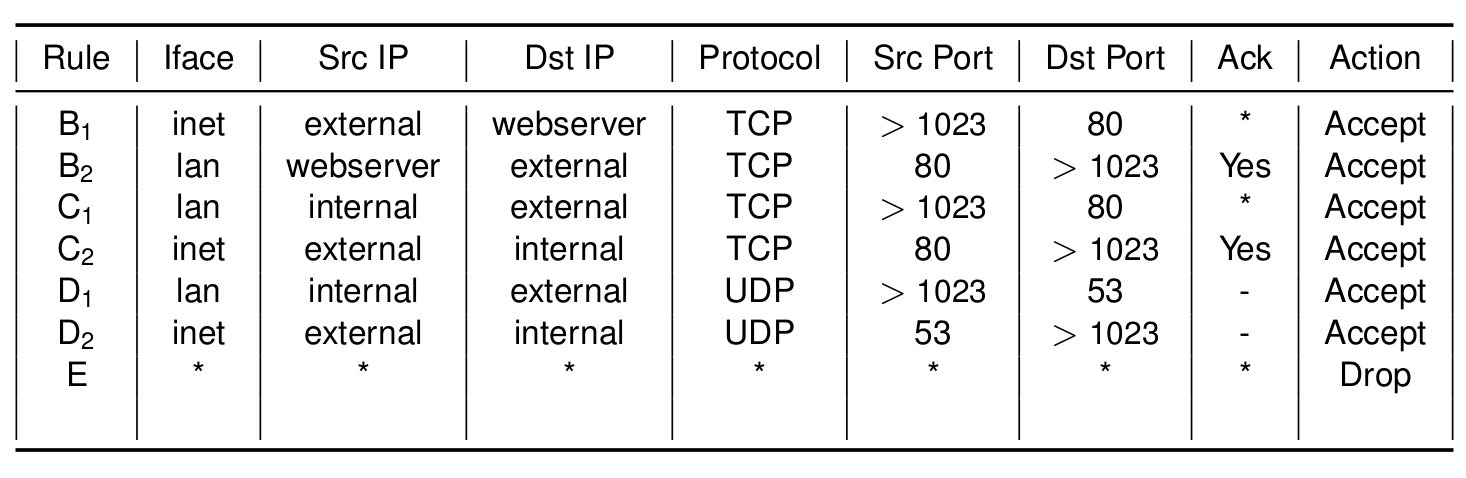
\includegraphics[width=.8\textwidth]{figures/stateless_firewall.png}
  \caption{Stateless Firewall Configuration}\label{fig:stateless_firewall}
\end{figure}

Stateless firewalls usually look at the ACK flag of TCP connection to determine approximately if connections are new or established.
When a SYN/ACK packet is sent as first packet of a connection, the firewall will pass it but the host will drop it if implement properly.

\subsubsection*{Spoofing Protection}
Spoofing is the forgery of IP addresses by filling the source IP field with another IP than one's own.
Spoofing protection then allows only IP addresses that belong to you on outgoing connections.
For incoming traffic this is more difficult since we can not determine where the packet actually came from so we are only able to block our and special purpose IPs.

\subsubsection*{Common Errors}
\begin{itemize}[noitemsep, topsep=0pt]
  \item How is your firewall management interface reachable?
  \item What is allowed over the Internet?
  \item IPv4 and IPv6?
  \item Outbound rule ANY? (c.f.\ spoofing)
  \item Policy’s vs. Firewalls understanding of Inbound and Outbound?
  \item Shadowing: unreachable firewall rules
\end{itemize}

\subsubsection*{What Firewalls cannot do}
\begin{itemize}[noitemsep, topsep=0pt]
  \item can’t protect against malicious insiders
  \item can’t protect against connections that don’t go through it
  \item can’t protect against completely new threats
  \item can’t fully protect against viruses
  \item does not perform cryptographic operations, e.g.\ message authentication
  \item can’t set itself up correctly
\end{itemize}

\subsubsection*{Bastion Hosts}
A bastion host is a host that is more exposed to the hosts of an external network than the other hosts of the network it protects.
When configuring, one should keep in mind that it might get compromised so do things like disabling SSH password login, do not allow it to sniff internal traffic or disable user accounts.

\subsubsection*{Firewall Architectures}
\begin{description}
  \item[Simple Packet Filter Architecture] Packet filtering is done through a filtering router or firewall with two interfaces.
    \begin{figure}[H]
      \centering
      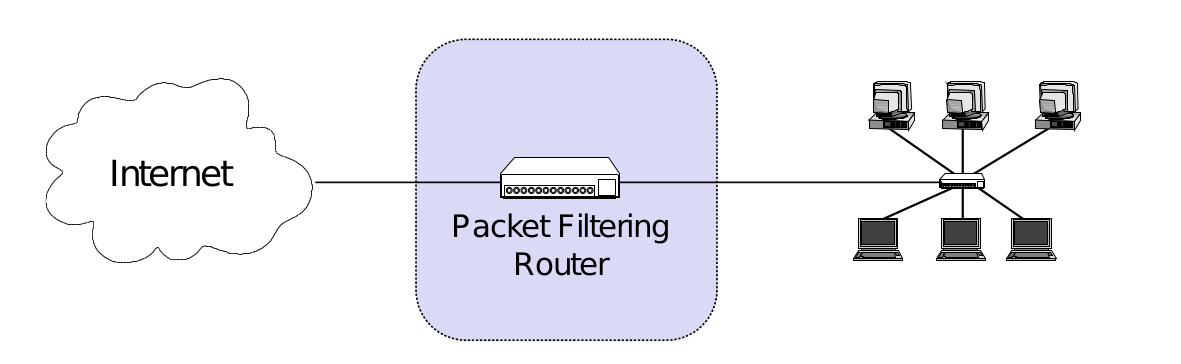
\includegraphics[width=.8\textwidth]{figures/firewall_simple_packet_filter_architecture.png}
    \end{figure}
  \item[Dual-Homed Host Architecture] The bastion host is part of two networks and is firewall and application proxy.
    Disadvantage: bastion host is bottleneck
    \begin{figure}[H]
      \centering
    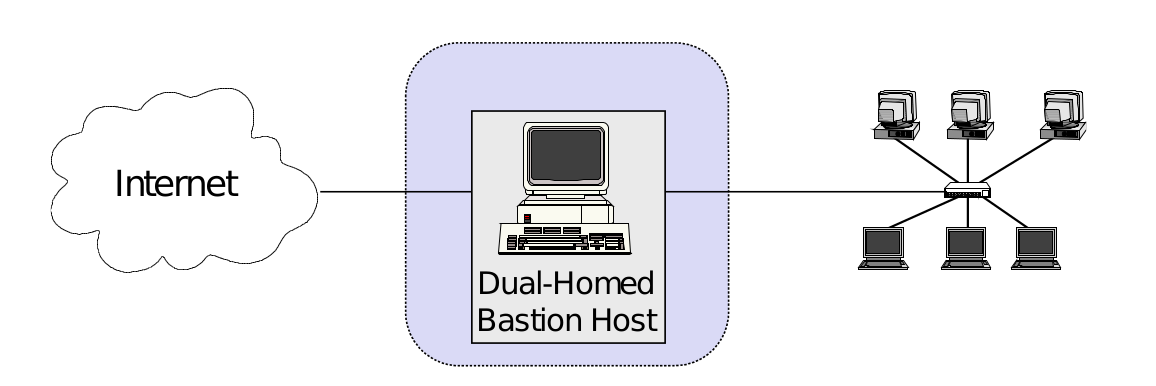
\includegraphics[width=.8\textwidth]{figures/firewall_dual-homed_host_architecture}
    \end{figure}
  \item[Screened Host Architecture] The bastion host is proxy, located in the internal network and thus protected by the firewall.
    \begin{figure}[H]
      \centering
      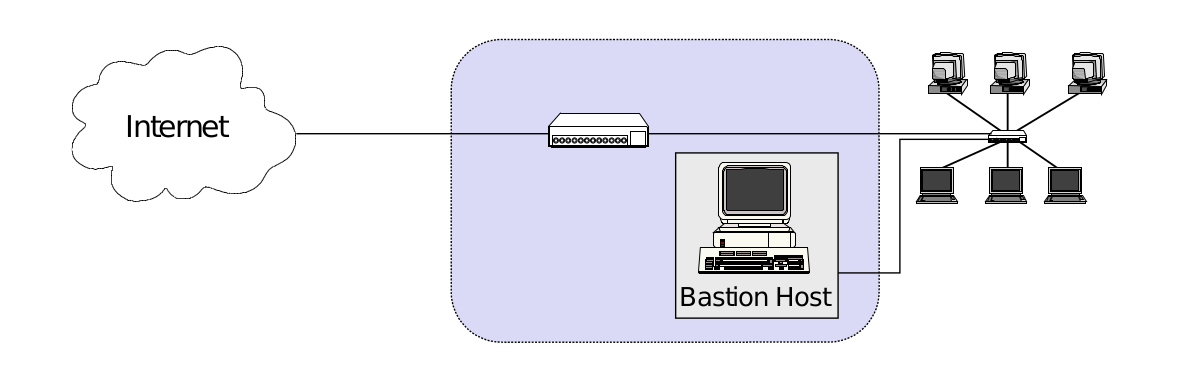
\includegraphics[width=.8\textwidth]{figures/firewall_screening_host_architecture.png}
    \end{figure}
  \item[Screened Subnet Architecture - DMZ] A demilitarized zone (DMZ) is configured hosting the bastion host (proxy) and publicly accessible servers.
    The second packet filter is an additional protection measurement in case the DMZ gets compromised.
    \begin{figure}[H]
      \centering
      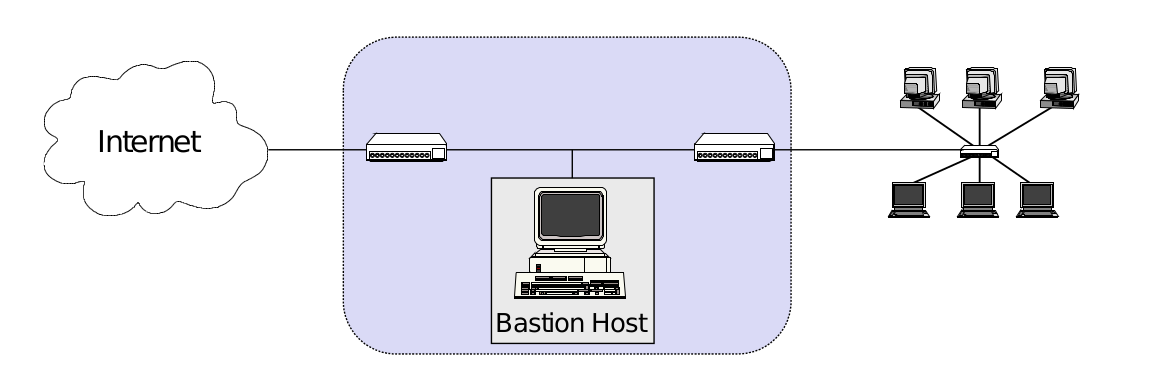
\includegraphics[width=.8\textwidth]{figures/firewall_screened_subnet_architecture.png}
    \end{figure}
\end{description}

\newpage

%!TEX root = ../report.tex

\section{TCP SYN Cookies}

\subsection{TCP SYN Flood Attack}
During an TCP SYN Flood Attack an attacker sends large amounts of packets with spoofed source addresses to the victim.
This fills up their connection table with half open connections (sequence numbers) which results in legitimate users not being able to establish new TCP connections.
A solution for this are TCP SYN cookies.

\subsection{TCP SYN Cookies}
TCP SYN Cookies are particularly chosen initial sequence numbers $\alpha = h(S_{SYN},K)$ where $K$ is a secret key, $S_{SYN}$ the source address of the SYN packet and $h$ a cryptographic hash function.
On arrival of the ACK message, Bob calculates $\alpha$ again and checks if the ACK number is correct ($\alpha + 1$).
This process is shown in Figure~\ref{fig:tcp_syn_cookies}.
\begin{figure}[h]
  \centering
  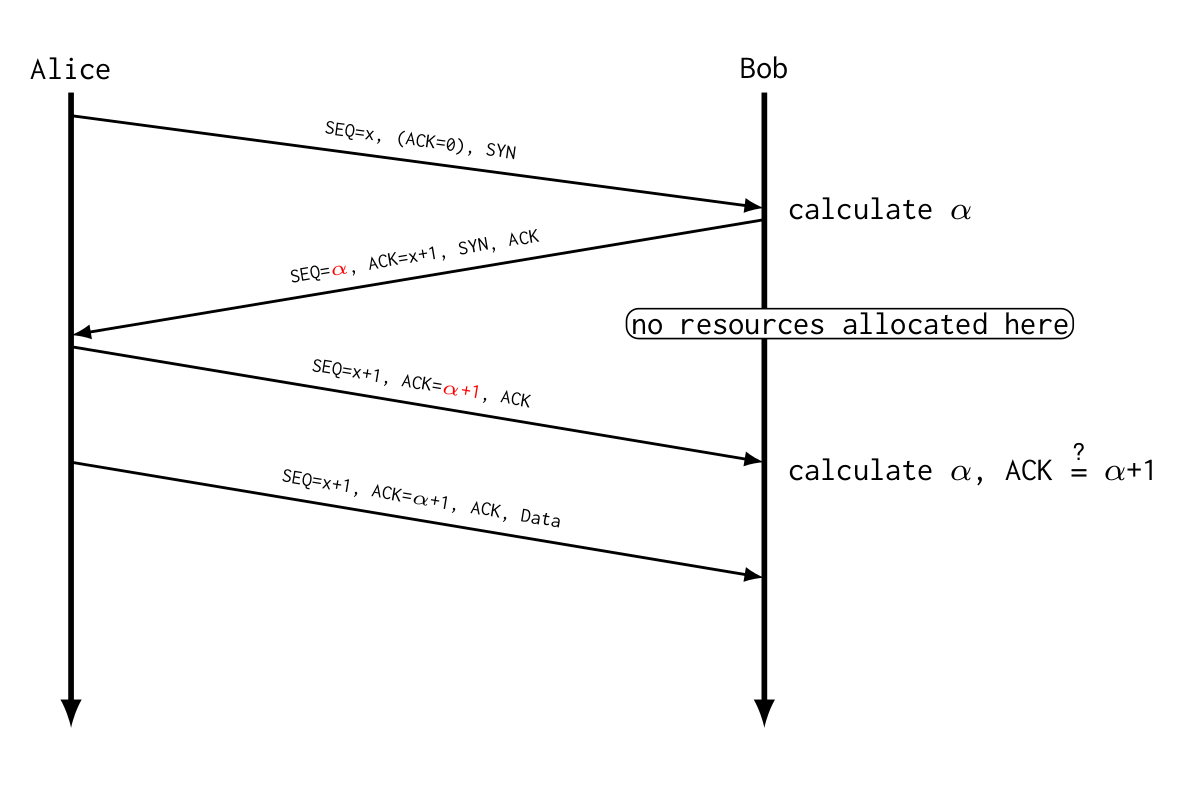
\includegraphics[width=.6\textwidth]{figures/tcp_syn_cookies.png}
  \caption{TCP SYN Cookies}\label{fig:tcp_syn_cookies}
\end{figure}

\begin{minipage}[t]{0.49\textwidth}
  \textbf{Pros}
  \begin{itemize}[topsep=0pt,noitemsep]
    \item No resource allocation after SYN packets
    \item Client does not have to be aware of the server using SYN cookies
    \item No changes in the TCP protocol necessary
  \end{itemize}
\end{minipage}
\begin{minipage}[t]{0.49\textwidth}
  \textbf{Cons}
  \begin{itemize}[topsep=0pt, noitemsep]
    \item Calculating $\alpha$ may be CPU consuming (Linux implementation: CPU local with high cashing efficiency)
    \item TCP options (like large windows size) cannot be negotiated (Linux implementation: window size hacked into cookie, SYN cookies only enabled if a threshold of connections is exceeded)
    \item Efficient implementations might be vulnerable to cryptoanalysis (Linux implementation: SHA used, counter updated every minute)
  \end{itemize}
\end{minipage}
\vspace{20pt}


\newpage

% Needs to be enabled when there are any references.
% \clearpage
% \addcontentsline{toc}{section}{\refname}
% \printbibliography

\end{document}
